\documentclass{article}
\usepackage{cite} % Add the cite package for citations

% Language setting
% Replace `english' with e.g. `spanish' to change the document language
\usepackage[english]{babel}

% Set page size and margins
% Replace `letterpaper' with `a4paper' for UK/EU standard size
\usepackage[letterpaper,top=2cm,bottom=2cm,left=3cm,right=3cm,marginparwidth=1.75cm]{geometry}

% Useful packages
\usepackage{amsmath}
\usepackage{graphicx}
\usepackage[colorlinks=true, allcolors=blue]{hyperref}

\title{Journal2}
\author{Raja Kantheti}

\begin{document}
\maketitle

\section{Introduction}
I am a master's student in Computer Science at UCCS. I want to choose the thesis path to satisfy the degree requirements. My expected course outcomes are to learn what it means to conduct research, how to write scientific papers, better articulate my ideas and evaluate their novelty, and write at least one paper of any type by the end of the semester.

I want to do my thesis on processor pipeline design, which would optimize branch prediction using additional prefetching and decoding units in parallel with the central decode unit. This pipeline could also mitigate SPECTRE attacks, which exploit Speculative execution. 

My eagerness to learn and grow is reflected in my goals for this course. I am determined to evaluate my thesis proposal, understand the necessary steps to evaluate the outcomes of my thesis, and grasp the elements of a successful proposal. I am also excited to challenge myself, to see if I have the stamina for long-term research and if this path is the right one for my career progression.

Some personal things about me outside of academia are that I like to be in solitude from time to time, lost in my thoughts and devices, contemplating meta-ethics, talking and debating with myself, and exploring all possibilities. The routines that would allow me to do this are my hobbies: Long walks and longer drives, camping alone, hiking in state/national parks, and this could be well out of the normalcy my other hobbies suggest, wood carving. 
% \begin{figure}[h]
% \centering
% 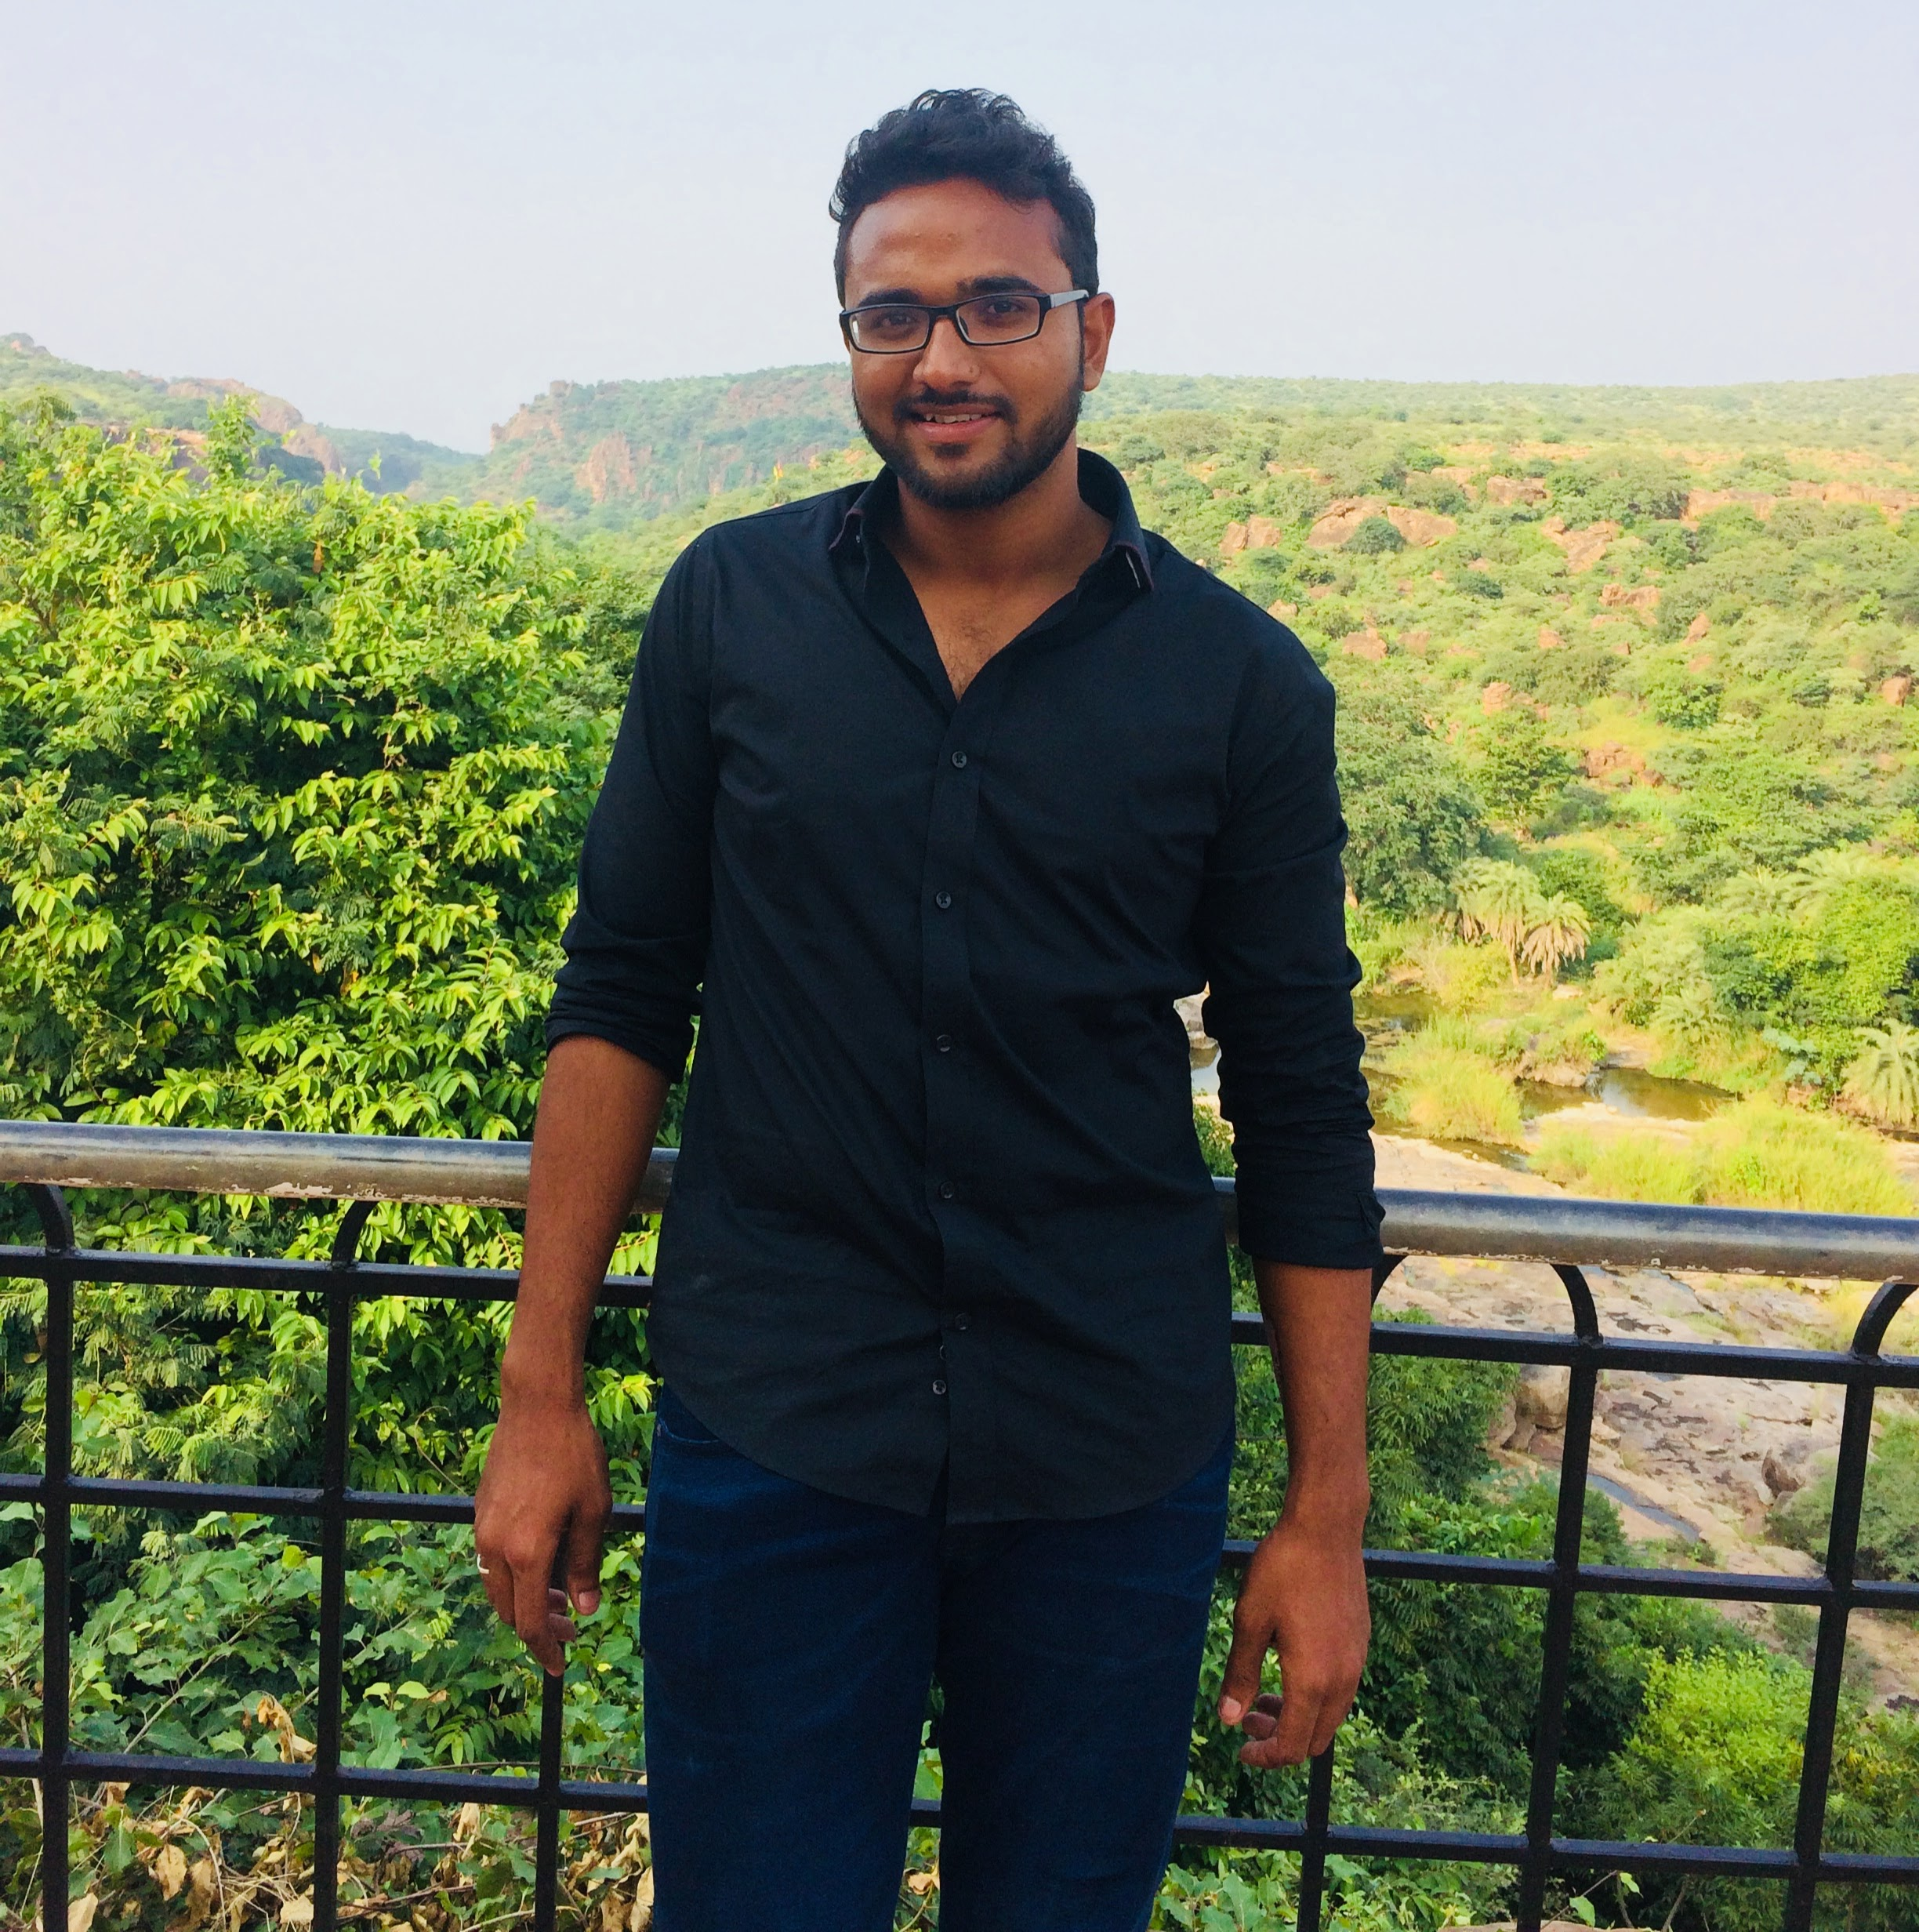
\includegraphics[width=0.25\linewidth]{IMG_1667.JPG}
% \caption{'tis I. }
% \end{figure}
\subsection[short]{Rationale on what was a good paper}
According to me, a good paper should question and delve into the fundamentals of its field by presenting a novel approach to understanding the core principles of Computer Science. It should provide proof of concept through unbiased experiments that reflect realistic scenarios, ensuring the integrity and applicability of the results. Additionally, the benchmarks or metrics used to quantify the findings must be relevant and appropriate, accurately measuring the impact and significance of the research conducted. 

A good paper should also be well-structured, with a clear introduction, methodology, results, and conclusion, guiding the reader through the research process. It should be concise, avoiding unnecessary jargon and complex language, making it accessible to a wide audience. Furthermore, a good paper should be well-referenced, citing relevant sources and acknowledging the contributions of other researchers in the field.

% \begin{figure}[h]
%       \centering
%       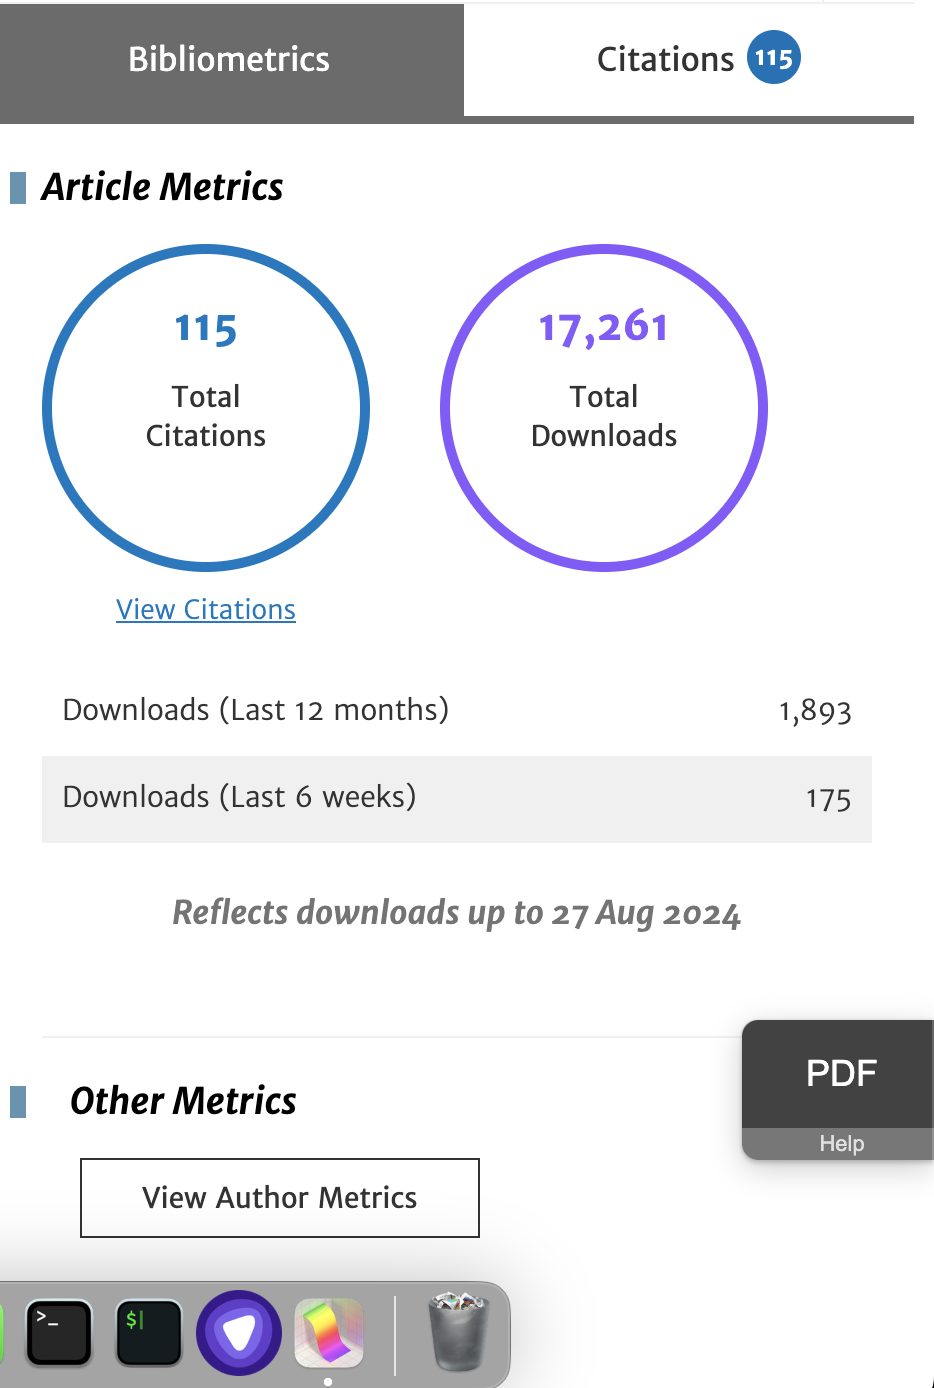
\includegraphics[width=0.25\linewidth]{Screenshot 2024-09-01 at 6.12.49 PM.png}
%       \caption{Paper: Spectre Attacks showcasing the relevance and citations. \cite{10.1145/3399742} }
% \end{figure}

\section{Tools}
I used Google Scholar and the ACM Digital Library to access and review research papers. These tools helped source recent, peer-reviewed articles. Google Scholar's comprehensive search and citation tracking features and the ACM Library's focused repository helped me find and analyze relevant studies on speculative execution and branch prediction. I faced challenges managing vast information and understanding complex technical details. I  refined my search terms, skimmed through abstracts for relevance, and used citation networks to identify key papers. 

As shown in the class, I was able to set alerts and refine my search results, and I was able to find more relevant papers to quantify and compare my results. I understood how the articles/papers are cataloged, and I also learned how to form a relevance threshold by which I can judge whether the paper would further the scope of my research. 

\bibliographystyle{alpha}
\bibliography{references}
\end{document}